\documentclass[12pt]{article}


% The default font size is 10pt; 11pt and 12pt are alternatives
%%%%%%%%%%%%%%%%%%%%%%%%%%%%%%%%%%%%%%%%%
% Professional Newsletter Template
% Structural Definitions File
% Version 1.0 (09/03/14)
%
% Created by:
% Vel (vel@latextemplates.com)
%
% This file has been downloaded from:
% http://www.LaTeXTemplates.com
%
% License:
% CC BY-NC-SA 3.0 (http://creativecommons.org/licenses/by-nc-sa/3.0/)
%
%%%%%%%%%%%%%%%%%%%%%%%%%%%%%%%%%%%%%%%%%

%----------------------------------------------------------------------------------------
%	REQUIRED PACKAGES
%----------------------------------------------------------------------------------------

\usepackage{graphicx} % Required for including images
\usepackage{microtype} % Improved typography
\usepackage{multicol} % Used for the two-column layout of the document
\usepackage{booktabs} % Required for nice horizontal rules in tables
\usepackage{wrapfig} % Required for in-line images
\usepackage{float} % Required for forcing figures not to float with the [H] parameter
\usepackage{ragged2e} 

%encoding
%--------------------------------------
\usepackage[utf8]{inputenc}
\usepackage[T1]{fontenc}
%--------------------------------------

%French-specific commands
%--------------------------------------
\usepackage[french]{babel}
\usepackage[autolanguage]{numprint}

%------------------------------------------------
%Hyphenation rules
%--------------------------------------
\usepackage{hyphenat}
\hyphenation{mathéma-tiques récu-pérer}
%--------------------------------------

% Fonts

%-\usepackage{charter} % Use the Charter font as the main document font
%-\usepackage{courier} % Use the Courier font for \texttt (monospaced) only
%-\usepackage[T1]{fontenc} % Use T1 font encoding

%------------------------------------------------
% List Separation

%-\usepackage{enumitem} % Required to customize the list environments
%-\setlist{noitemsep,nolistsep} % Remove spacing before, after and within lists for a compact look

%------------------------------------------------
% Figure and Table Caption Styles

\usepackage{caption} % Required for changing caption styles
\captionsetup[table]{labelfont={bf,sf},labelsep=period,justification=justified} % Specify the table caption style
\captionsetup[figure]{labelfont={sf,bf},labelsep=period,justification=justified, font=small} % Specify the figure caption style
\setlength{\abovecaptionskip}{10pt} % Whitespace above captions

%------------------------------------------------
% Spacing Between Paragraphs

\makeatletter
\usepackage{parskip}
\setlength{\parskip}{6pt}
\newcommand{\@minipagerestore}{\setlength{\parskip}{6pt}}
\makeatother

%----------------------------------------------------------------------------------------
%	PAGE MARGINS AND SPACINGS
%----------------------------------------------------------------------------------------

\textwidth = 7 in % Text width
\textheight = 10 in % Text height
\oddsidemargin = -18pt % Left side margin on odd pages
\evensidemargin = -18pt % Left side margin on even pages
\topmargin = -36pt % Top margin
\headheight = 0pt % Remove the header by setting its space to 0
\headsep = 0pt % Remove the space between the header and top of the page
\parskip = 4pt % Space between paragraph
\parindent = 0.0in % Paragraph indentation
\pagestyle{empty} % Disable page numbering

%----------------------------------------------------------------------------------------
%	COLORS
%----------------------------------------------------------------------------------------

\usepackage[dvipsnames,svgnames]{xcolor} % Required to specify custom colors

\definecolor{altncolor}{rgb}{.8,0,0} % Dark red
%\definecolor{altncolor}{rgb}{.2,.4,.8} % Dark blue
%\definecolor{altncolor}{rgb}{.84,.16,.16} % Red

\usepackage[colorlinks=true, linkcolor=altncolor, anchorcolor=altncolor, citecolor=altncolor, filecolor=altncolor, menucolor=altncolor, urlcolor=altncolor]{hyperref} % Use the color defined above for all links

%----------------------------------------------------------------------------------------
%	BOX STYLES
%----------------------------------------------------------------------------------------

\usepackage[framemethod=TikZ]{mdframed}% Required for creating boxes
\mdfdefinestyle{sidebar}{
    linecolor=black, % Outer line color
    outerlinewidth=0.5pt, % Outer line width
    roundcorner=0pt, % Amount of corner rounding
    innertopmargin=10pt, % Top margin
    innerbottommargin=10pt, % Bottom margin
    innerrightmargin=10pt, % Right margin
    innerleftmargin=10pt, % Left margin
    backgroundcolor=white, % Box background color
    frametitlebackgroundcolor=white, % Title background color
    frametitlerule=false, % Title rule - true or false
    frametitlerulecolor=white, % Title rule color
    frametitlerulewidth=0.5pt, % Title rule width
    frametitlefont=\Large, % Title heading font specification
    font=\small
}

\mdfdefinestyle{intextbox}{
    linecolor=black, % Outer line color
    outerlinewidth=0.5pt, % Outer line width
    roundcorner=10pt, % Amount of corner rounding
    innertopmargin=7pt, % Top margin
    innerbottommargin=7pt, % Bottom margin
    innerrightmargin=7pt, % Right margin
    innerleftmargin=7pt, % Left margin
    backgroundcolor=white, % Box background color
    frametitlebackgroundcolor=white, % Title background color
    frametitlerule=false, % Title rule - true or false
    frametitlerulecolor=white, % Title rule color
    frametitlerulewidth=0.5pt, % Title rule width
    frametitlefont=\Large % Title heading font specification
}

%----------------------------------------------------------------------------------------
%	HEADING STYLE
%----------------------------------------------------------------------------------------

\newcommand{\heading}[2]{ % Define the \heading command
\vspace{#2} % White space above the heading
{\begin{center}\Large\textbf{#1}\end{center}} % The heading style
\vspace{#2} % White space below the heading
}

\newcommand{\BackToContents}{\hyperlink{contents}{{\small Back to Contents}}} % Define a command for linking back to the contents of the newsletter






%%% ---------------
%%% DEFINITIONS
%%% ---------------

% Define separators
\newcommand{\HorRule}[1]{\noindent\rule{\linewidth}{#1}} % Creating a horizontal rule
\newcommand{\SepRule}{\noindent							 % Creating a separator
						\begin{center}
							\rule{250pt}{1pt}
						\end{center}
						}

% Define Title en News input
\newcommand{\JournalName}[1]{%
		\begin{center}
			\Huge \usefont{T1}{QTCaligulatype}{m}{n}
			#1%
		\end{center}
		\par \normalsize \normalfont}

\newcommand{\JournalIssue}[1]{%
		\hfill \textsc{\mydate \today, No #1}
		\par \normalsize \normalfont}

\newcommand{\NewsItem}[1]{%
		\usefont{T1}{augie}{m}{n}
		\large #1 \vspace{4pt}
		\par \normalsize \normalfont}

\newcommand{\NewsAuthor}[1]{%
			\hfill by \textsc{#1} \vspace{4pt}
			\par \normalfont}
 % Include the document which specifies all packages and structural customizations for this template

\begin{document}


%----------------------------------------------------------------------------------------
%	HEADER IMAGE
%----------------------------------------------------------------------------------------

% Title
% -----
\JournalName{\Huge\textbf {GDPR FINES NEWSLETTER}}
\noindent\HorRule{3pt} \\[-0.75\baselineskip]
\HorRule{1pt}

\vspace{0.5cm}
	\SepRule
\vspace{0.5cm}


%General Statistic
\NewsItem{\raggedright{\LARGE GDPR Fines Overview}}
\justify
The General Data Protection Regulation 2016/679 is a regulation in EU law on data protection and privacy in the European Union and the European Economic Area. \\
\textbf{530} fines have been given out until today.
The overall cumulative total of data protection fines now stands at \textbf{275 187 314€}.


\begin{figure}
	[H]\centering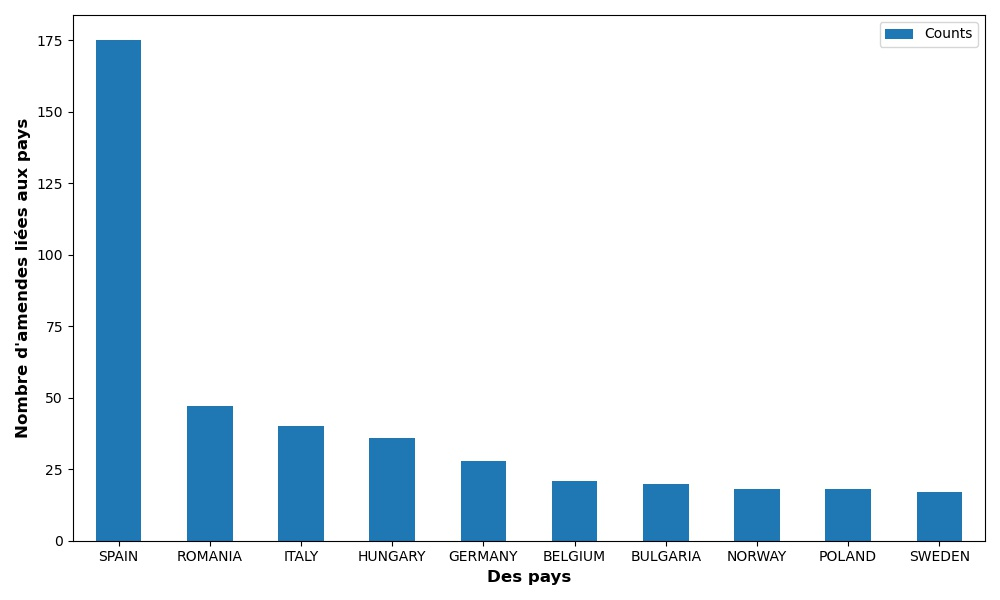
\includegraphics[width=0.7\linewidth]{graphs/top10_countries}
      \caption{Top 10 EU Countries with the highest number of fines }
\end{figure}
\begin{figure}
	[H]\centering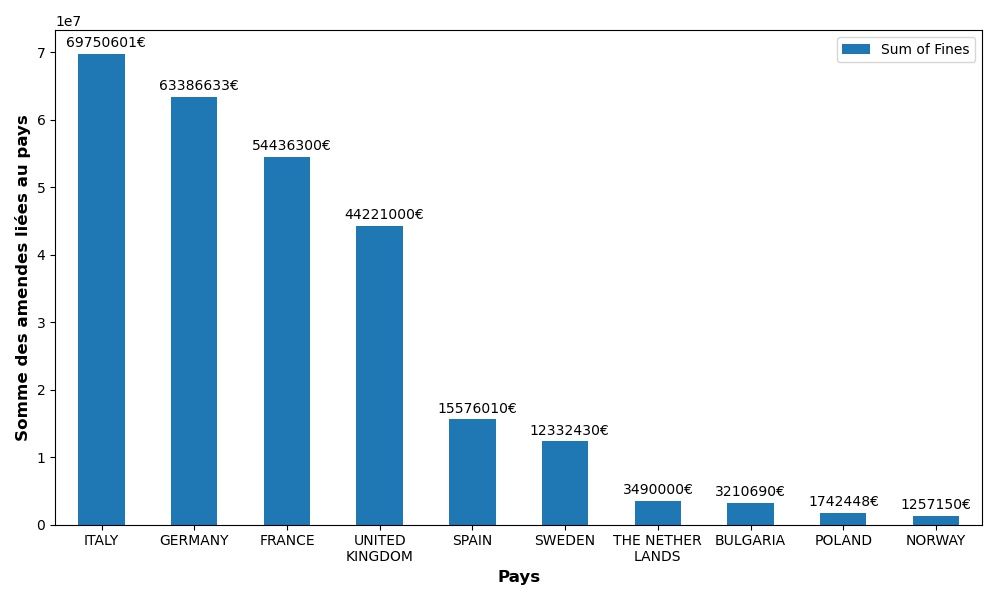
\includegraphics[width=0.7\linewidth]{graphs/top10_countries_fines}
	\caption{Top 10 EU Countries with the highest sum of fines}
 \end{figure}


\newpage

	\begin{multicols}{2}
	\begin{figure}
		[H]\centering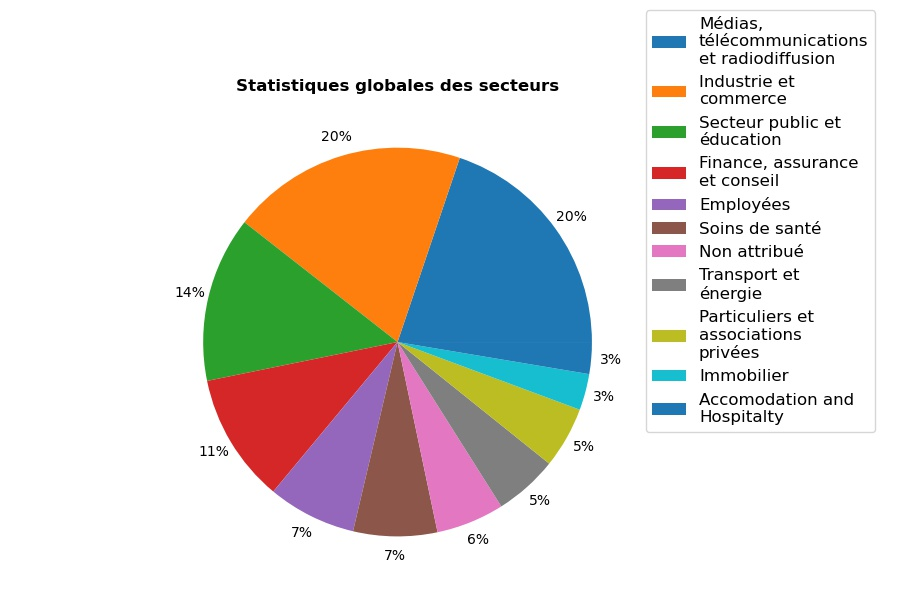
\includegraphics[width=1.0\linewidth]{graphs/sector_data}
		\caption{Top 10 Sectors on piechart with the highest number of fines}
	\end{figure}
	\begin{figure}
		[H]\centering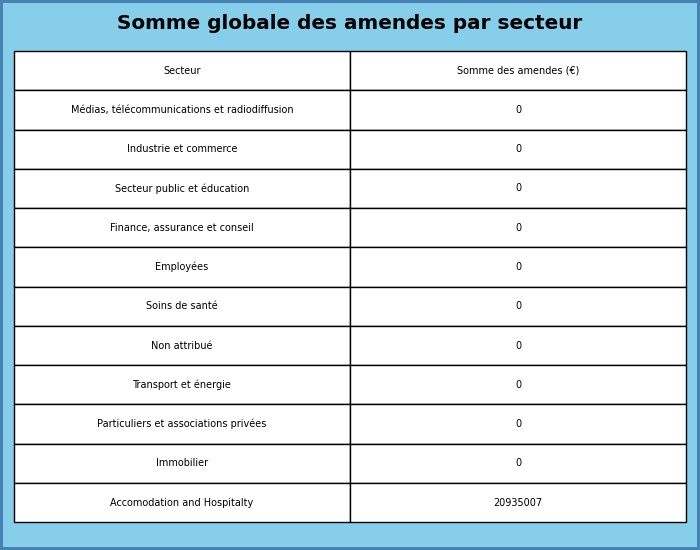
\includegraphics[width=1\linewidth]{graphs/sector_data_fines}
		\caption{Top 10 Sectors with the highest amount of fines}
	 \end{figure}
	
	\end{multicols}
	
	
	
	\begin{figure}
		[H]\centering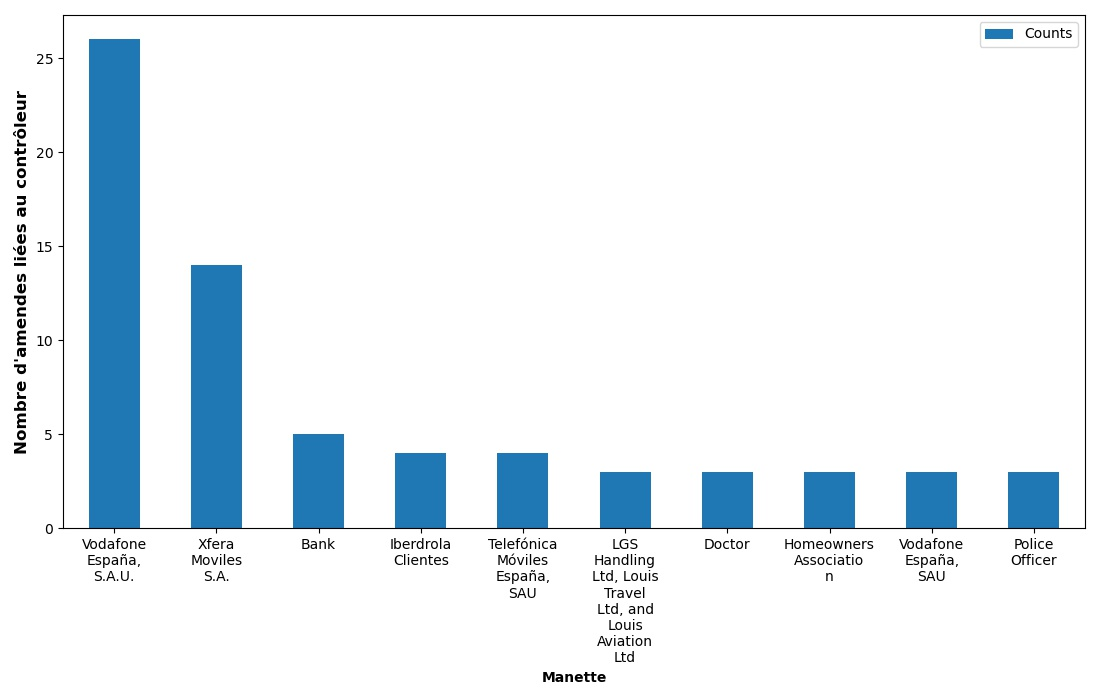
\includegraphics[width=0.6\linewidth]{graphs/top10_controller}
		\caption{Top 10 Companies with the highest number of fines}
	\end{figure}
	
	\begin{figure}
		[H]\centering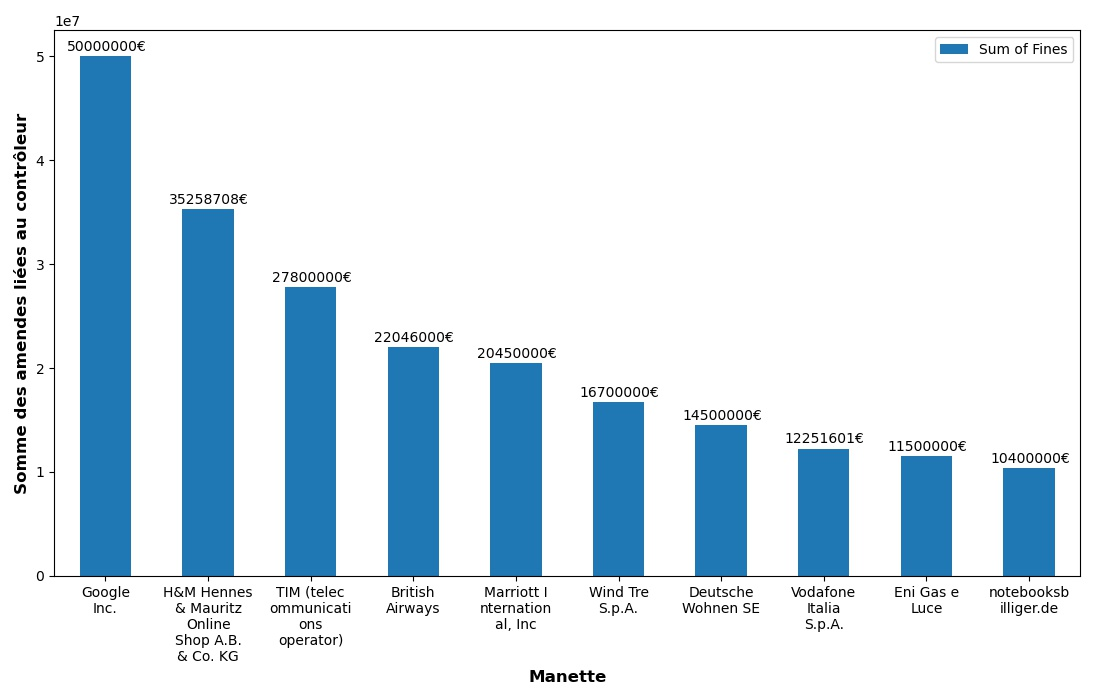
\includegraphics[width=0.6\linewidth]{graphs/top10_controller_fines}
		\caption{Top 10 Companies with the highest amount of fines}
	 \end{figure}



\newpage


	\begin{multicols}{2}
	\begin{figure}
		[H]\centering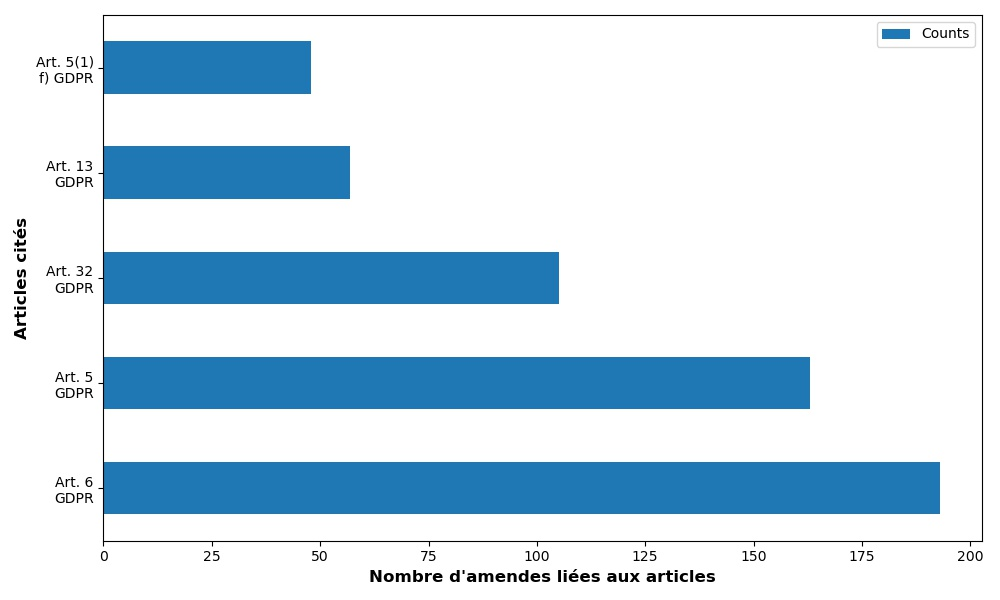
\includegraphics[width=1\linewidth]{graphs/top10_quoted} 
		\caption{Top 5 Quoted Articles with the highest number of fines}
	\end{figure}
	\begin{figure}
		[H]\centering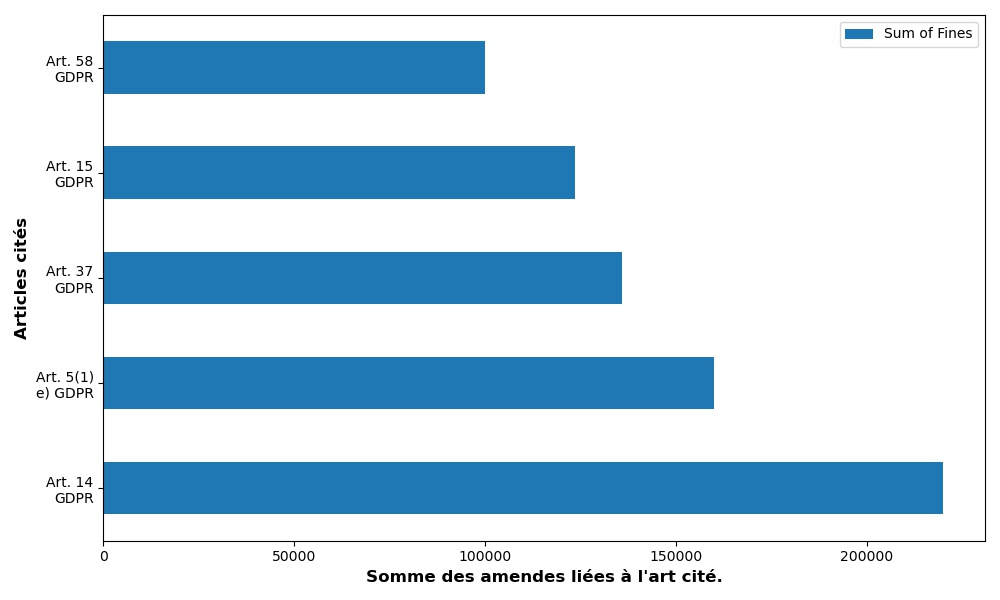
\includegraphics[width=1\linewidth]{graphs/top10_quoted_fines} 
		\caption{Top 5  Quoted Articles with the highest amount of fines}
	\end{figure}
	\end{multicols}
	
	
	\NewsItem{\raggedright{\LARGE Analysis on GDPR enforcement over years}}
	\begin{figure}
		[H]\centering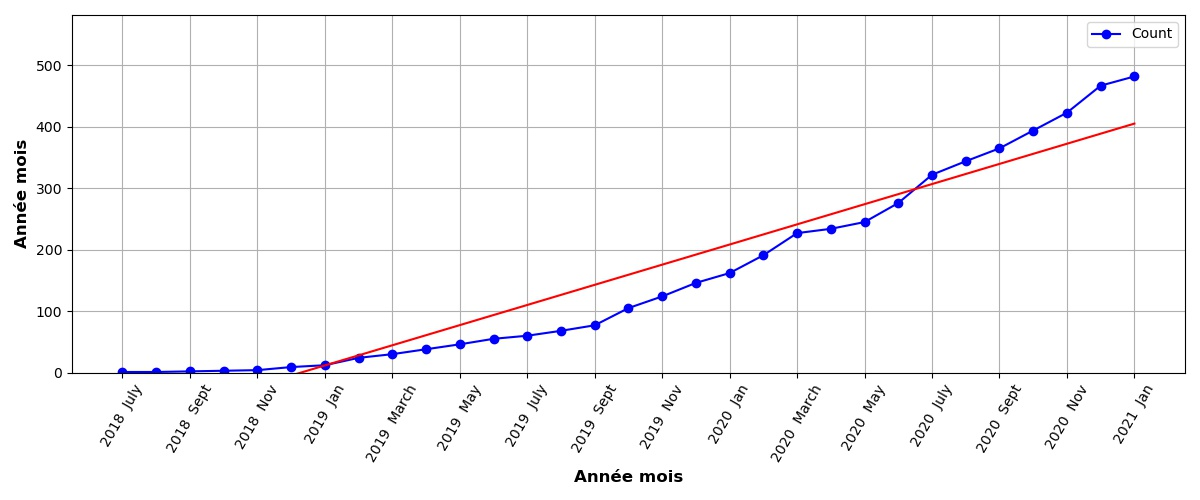
\includegraphics[width=0.8\linewidth]{graphs/acc_nb_cases_graph}
		\caption{Overall Number of Fines (cumulative) }
	\end{figure}
	
	\begin{multicols}{2}
	\begin{figure}
		[H]\centering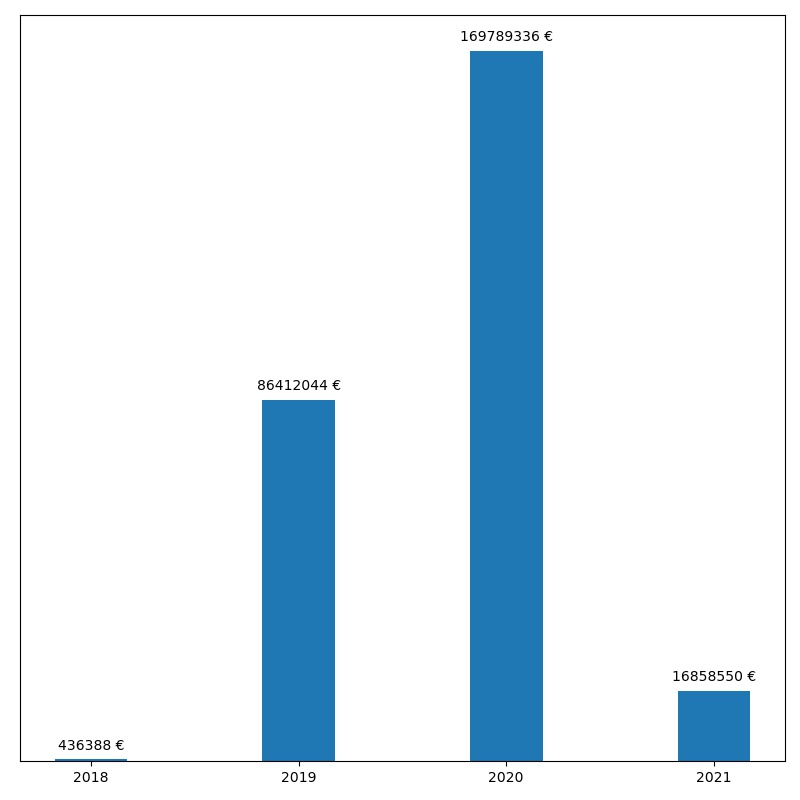
\includegraphics[width=1.0\linewidth]{graphs/SumOfFinesperYear}
		\caption{Overall Amount of Fines per year }
	 \end{figure}
\justify
	GDPR enforcement has accelerated since the first few years, both on the number of enforcement cases as well as the sum of fines. Public awareness and media coverage on privacy and data protection have increased over the years too. However, GDPR is at the risk of failing. According to a research from Brave, this is due to the Data Protection Authorities(DPA) not giving enough human and financial resources to perform their tasks. Only 6 national DPAs have more than 10 specialist tech investigation staff. Half of all national DPAs receive small (€5 million or less) annual budgets from their governments.
	\end{multicols}



\newpage



%Particular Year Statistic
\NewsItem{\raggedright{\LARGE GDPR fines overview in 2018}}

	\begin{multicols}{2}
	
	In 2018, there have been \textbf{12} fines.
	The cumulative total of data protection fines for 2018 now stands at \textbf{458 688€}.
	
	\begin{figure}[H]
	\centering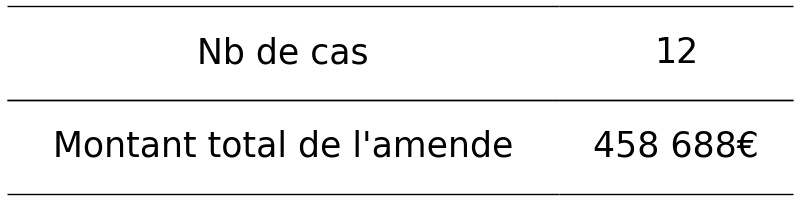
\includegraphics[width=1\linewidth]{graphs/counter_year}
	\end{figure}


	The GPDR fines for 2018 break down for each months as follow :

	\begin{figure}
	[H]\centering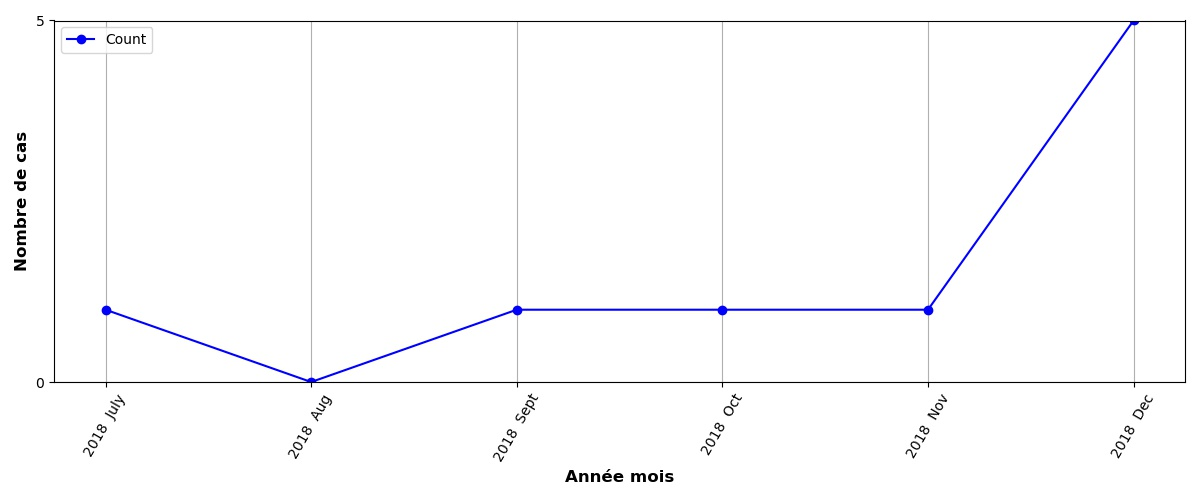
\includegraphics[width = 1.2\linewidth]{graphs/NbFinesPerMonth_year_graph}
	\caption{Small Overview over months in 2018}
	\end{figure}

	\end{multicols}


	\begin{figure}
		[H]\centering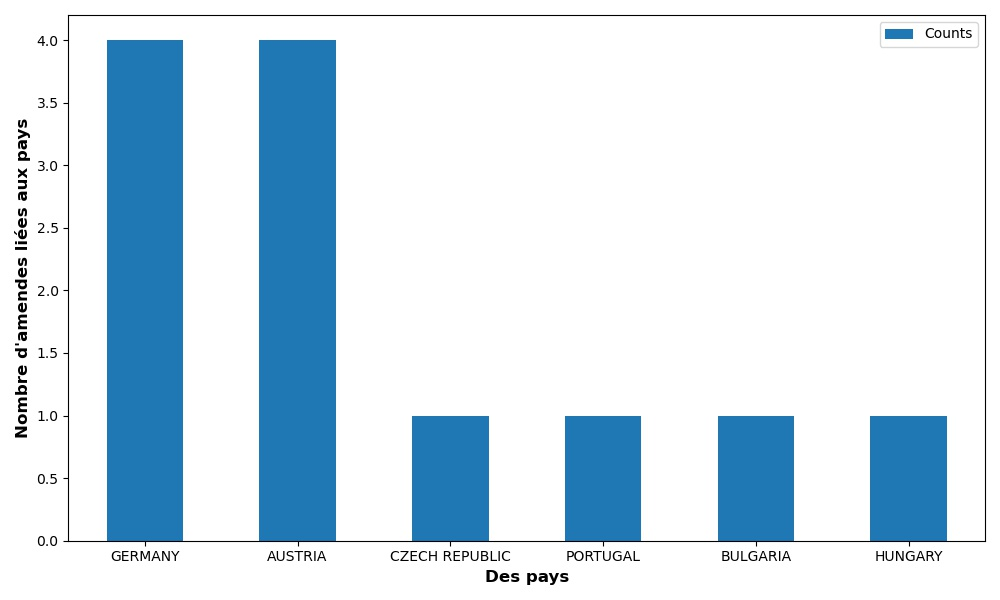
\includegraphics[scale=.5]{graphs/top10_countries_year}
		\caption{Top 10 EU Countries with the highest number of fines in 2018}
	\end{figure}
	\begin{figure}
		[H]\centering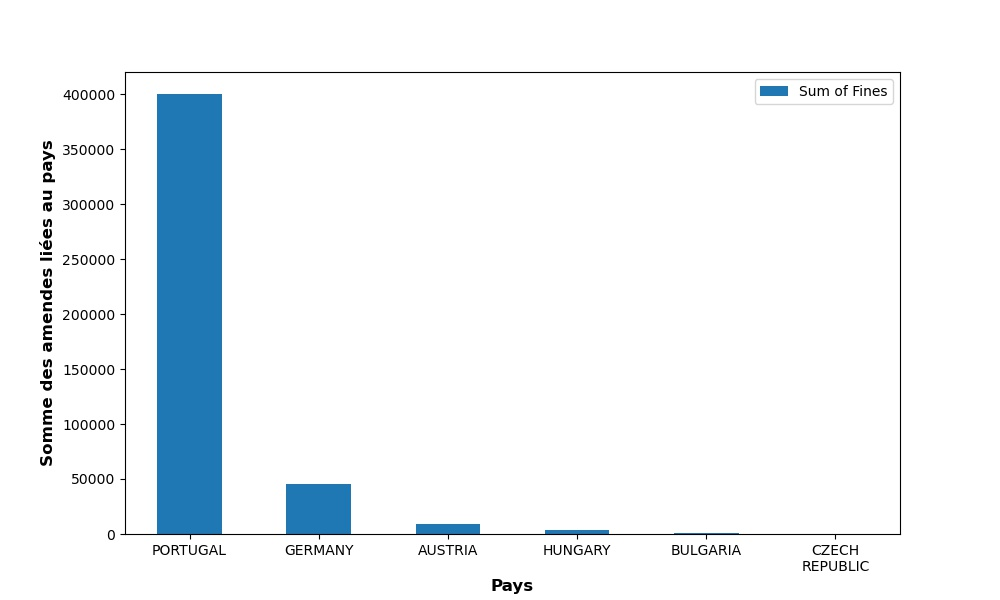
\includegraphics[scale=.5]{graphs/top10_countries_year_fines}
		\caption{Top 10 EU Countries with the highest sum of fines in 2018}
	\end{figure}

\newpage
\justify
	\begin{multicols}{2}
	\heading{3 most recent fines in 2018}{3 pt}
		\begin{itemize}
			\item \textbf{2018-12-20} \newline
			2,200€ fine issued in AUSTRIA to Private person.
			\newline
			The fine was imposed against a private person who was using CCTV at his home. The video surveillance covered areas which are intended for the general use of the residents of the multi-party residential complex, namely: parking lots, sidewalks, courtyard, garden and access areas to the residential complex; in addition, the video surveillance covered garden areas of an adjacent property. The video surveillance subject of the proceedings is therefore not limited to areas which are under the exclusive power of control of the controller. Video surveillance is therefore not proportionate to the purpose and not limited to what is necessary. The video surveillance records the hallway of the house and films residents entering and leaving the surrounding apartments, thereby intervening in their highly personal areas of life without the consent to record their image data. The video surveillance was not properly indicated.
			\newline
			\href{https://www.ris.bka.gv.at/Dokumente/Dsk/DSBT_20181220_DSB_D550_037_0003_DSB_2018_00/DSBT_20181220_DSB_D550_037_0003_DSB_2018_00.pdf}{More Info}
			\vspace{1cm}
	
			\item \textbf{2018-12-18} \newline
			3,200€ fine issued in HUNGARY to Unknown.
			\newline
			The fine was imposed for (i) not providing a data subject with CCTV recordings, (ii) not retaining recordings for further use by the data subject, and (iii) not informing the data subject about his right to lodge a complaint to the supervisory authority.
			\newline
			\href{https://www.naih.hu/files/NAIH-2018-5559-H-hatarozat.pdf}{More Info}
			\vspace{1cm}
	
			\item \textbf{2018-12-17} \newline 5,000€ fine issued in GERMANY to Kolibri ImageRegina und Dirk Maass GbR
			\newline
			Please note: According to our information this fine has been withdrawn in the meantime. Kolibri Image had send a request to the Data Protection Authority of Hessen asking how to deal with a service provider who does not want to sign a processing agreement. After not answering Kolibri Image in more detail, the case was forwarded to the locally responsible Data Protection Authority of Hamburg. This Authority then fined Kolibri Image as controller for not having a processing agreement with the service provider. Kolibri Image has stated that they will challenge the decision in front of court since they are of the opinion that the service provider does not act as a processor.
			\newline
			\href{https://www.heise.de/newsticker/meldung/DSGVO-5000-Euro-Bussgeld-fuer-fehlenden-Auftragsverarbeitungsvertrag-4282737.html}{More Info}
		\end{itemize}
	\end{multicols}

\newpage
\justify
	\begin{multicols}{2}
	\raggedright\heading{Notable fines in 2018}{3 pt}
		\begin{itemize}
			\item The \textbf{largest} fine of 2018 - \textbf{400000 €} - was issued in PORTUGAL to Public Hospital.
			\newline
			\textbf{Summary} : Investigation revealed that the hospital’s staff, psychologists, dietitians and other professionals had access to patient data through false profiles.  The profile management system appeared deficient – the hospital had 985 registered doctor profiles while only having 296 doctors.  Moreover, doctors had unrestricted access to all patient files, regardless of the doctor’s specialty.
			\newline
			\href{https://www.cnpd.pt/bin/decisoes/Delib/20_984_2018.pdf}{More info}
			\vspace{1cm}
		
			\item The \textbf{lowest} fine of 2018 - \textbf{300 €} - was issued in  to Private car owner.
			\newline
			\textbf{Summary} : A Dashcam was unlawfully used.
			\newline
			\href{https://www.ris.bka.gv.at/Dokumente/Dsk/DSBT_20180927_DSB_D550_084_0002_DSB_2018_00/DSBT_20180927_DSB_D550_084_0002_DSB_2018_00.pdf}{More info}
		\end{itemize}
	\end{multicols}


\newpage

	
	\begin{multicols}{2}
	\begin{figure}
		[H]\centering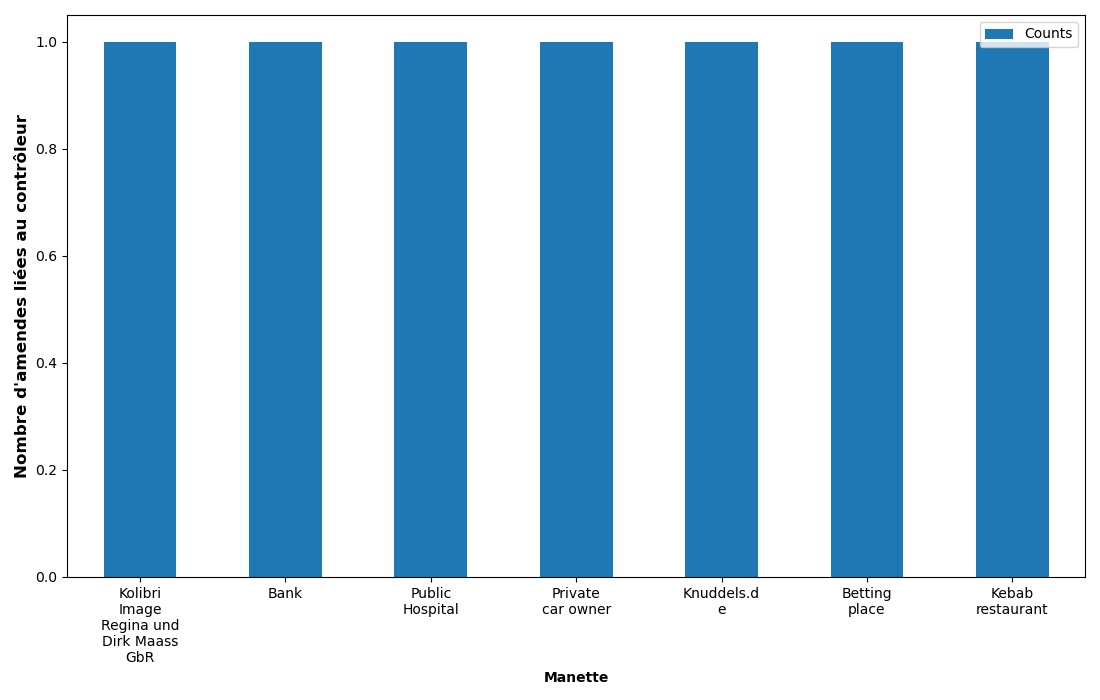
\includegraphics[width=1.0\linewidth]{graphs/top10_controller_year}
		\caption{Top 10 Companies with the highest number of fines in 2018}
	\end{figure}
	\begin{figure}
		[H]\centering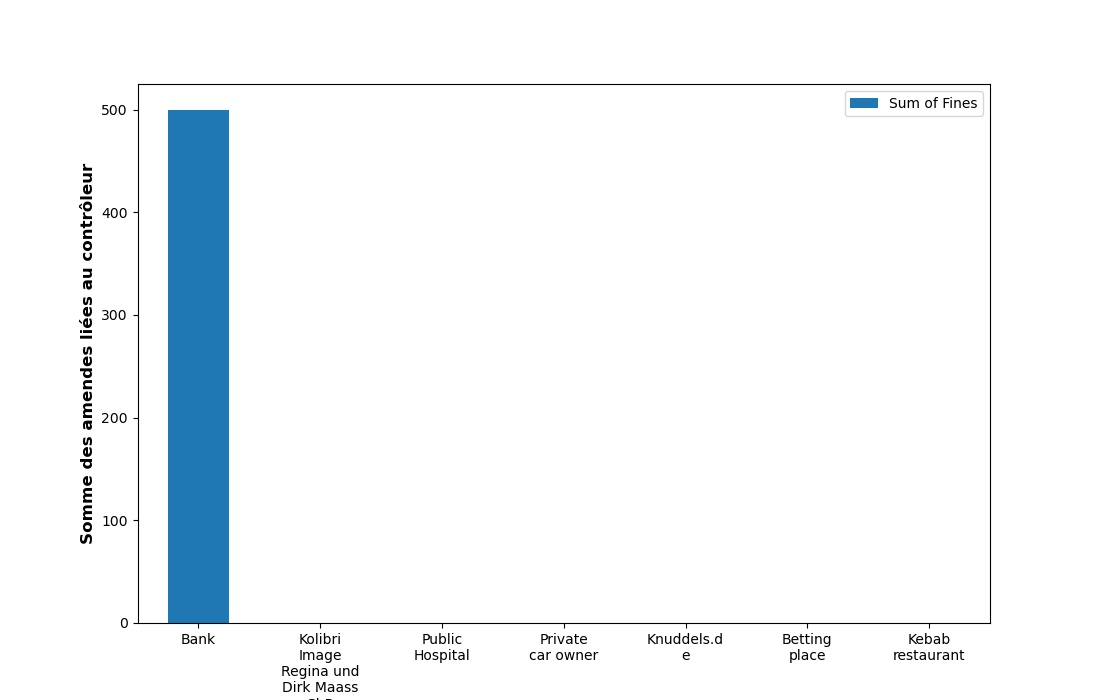
\includegraphics[width=1\linewidth]{graphs/top10_controller_year_fines}
		\caption{Top 10 Companies with the highest  amount of fines in 2018}
	 \end{figure}
	
	\end{multicols}


		
	\begin{multicols}{2}
	\begin{figure}
		[H]\centering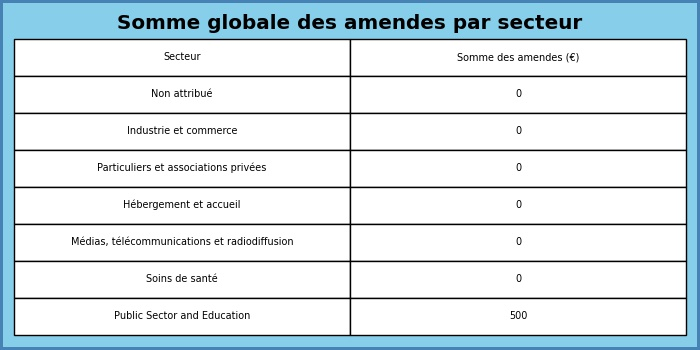
\includegraphics[width=1.0\linewidth]{graphs/sector_data_year_fines}
		\caption{Top 10 Sectors on piechart with the highest number of fines in 2018}
	\end{figure}
	\begin{figure}
		[H]\centering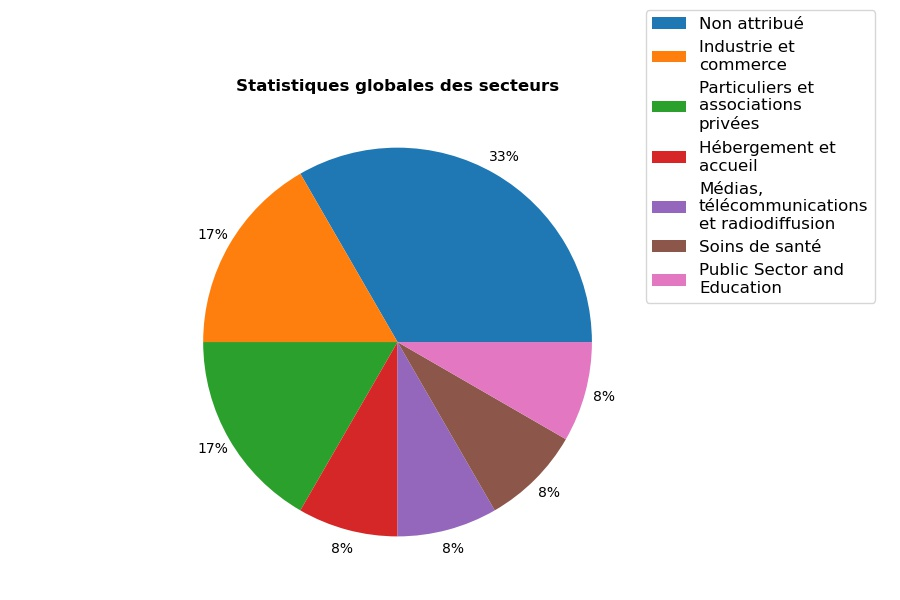
\includegraphics[width=1\linewidth]{graphs/sector_data_year}
		\caption{Top 10 Sectors with the highest amount of fines in 2018}
	 \end{figure}
	
	\end{multicols}

	\begin{multicols}{2}
	\begin{figure}
		[H]\centering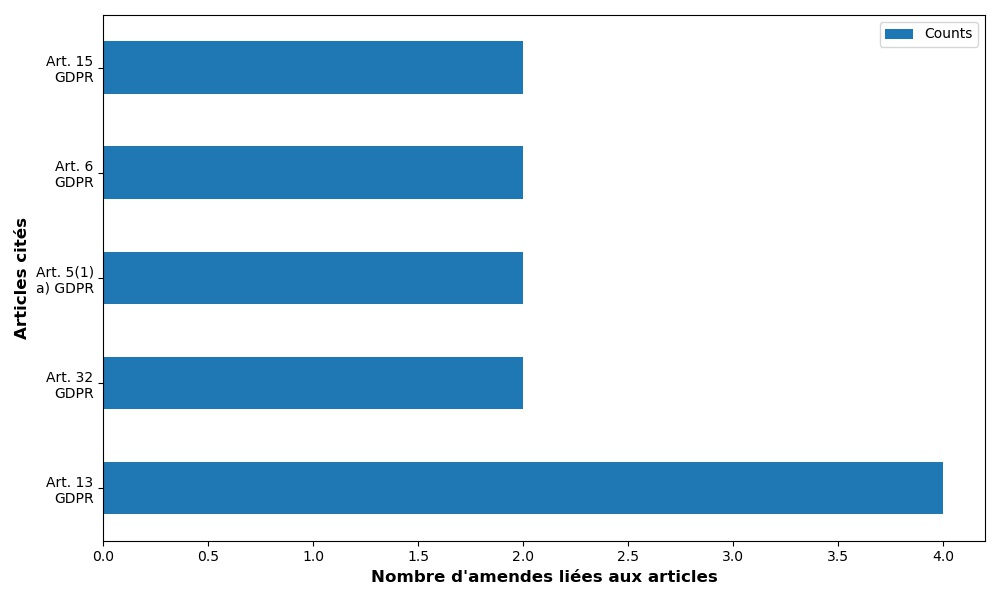
\includegraphics[width=1.0\linewidth]{graphs/top10_quoted_year}
		\caption{Top 10 Quoted Article with the highest number of fines in 2018}
	\end{figure}
	\begin{figure}
		[H]\centering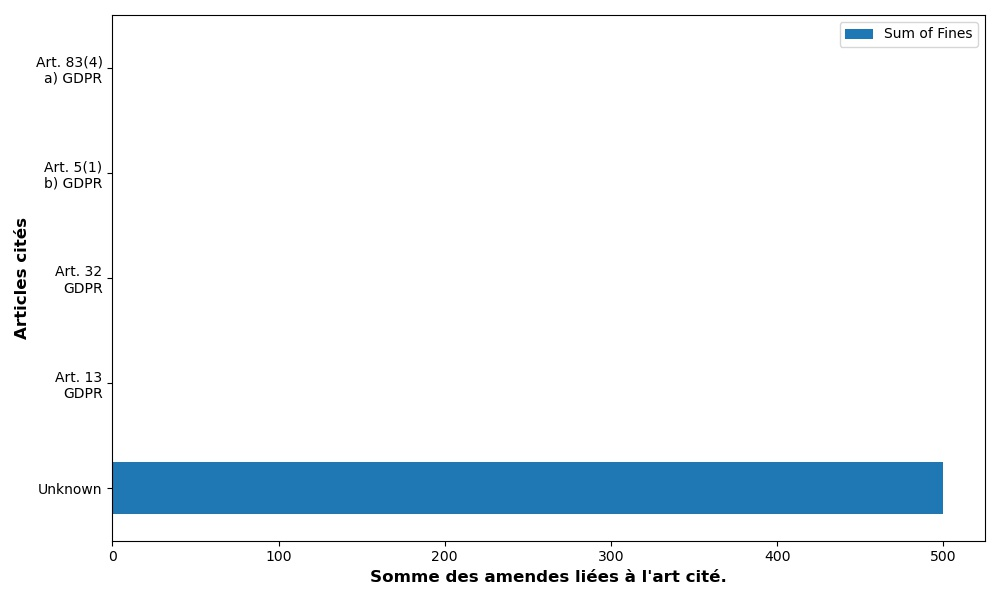
\includegraphics[width=1\linewidth]{graphs/top10_quoted_year_fines}
		\caption{Top 10 Quoted Article with the highest amount of fines in 2018}
	 \end{figure}
	
	\end{multicols}









\vspace*{\fill}
\textbf{References:}\\
\href{https://www.enforcementtracker.com}{https://www.enforcementtracker.com}\\
\href{https://brave.com/wp-content/uploads/2020/04/Brave-2020-DPA-Report.pdf}{https://brave.com/wp-content/uploads/2020/04/Brave-2020-DPA-Report.pdf}\\
\href{https://arxiv.org/pdf/2011.00946.pdf}{https://arxiv.org/pdf/2011.00946.pdf}


\end{document}